\chapter{Metodología}\label{chapter:metodologia}

La naturaleza de este proyecto implica hacer cambios constantemente, ya sea por los fallos producidos durante el desarrollo, por la necesidad de estar continuamente probando distintos algoritmos y evaluar si son adecuados, o simplemente por querer hacer mejoras en el diseño del producto en general. Es por ello que se exige una metodología flexible, por lo que la metodología ágil ha sido la más adecuada.

\begin{figure}[H]
    \centering
    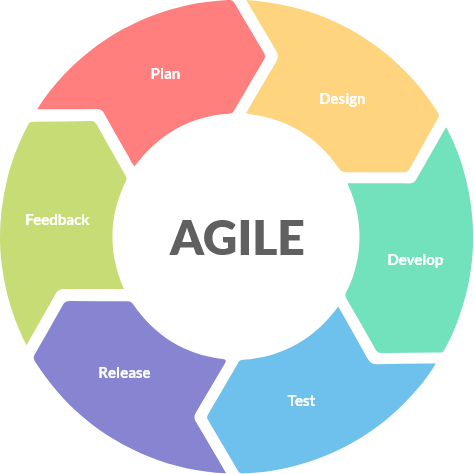
\includegraphics[width=8cm]{figures/agile.png}
    \caption[Ciclo de desarrollo ágil]{Ciclo de desarrollo ágil (Fuente: \parencite{agile-figure})}
    \label{agile}
\end{figure}

Siguiendo la metodología ágil, la idea ha sido que durante el trascurso del TFG se fuera definiendo periódicamente (cada una o dos semanas) un pequeño ciclo de trabajo, consistente en diseñar, implementar y probar una funcionalidad.

Para adaptarse a esta metodología, se han ido haciendo reuniones periódicas con el director, con la finalidad de verificar que el proyecto estuviera progresando correctamente, recibiendo \emph{feedback} e indicaciones, y que cumpliera con las competencias técnicas que se exigen.

\section{Herramientas}

Para hacer el seguimiento de todas las tareas que han surgido a lo largo del desarrollo de este proyecto, así como permitir una clara visualización de su estado, se ha utilizado la aplicación \emph{Trello}, la cual permite la creación de tareas en forma de bloques cuyos estados se pueden distinguir entre pendientes, en proceso o finalizados.

Además, con la finalidad de mantener un control de versiones, guardar copias de seguridad y compartir el código con el director del proyecto, se ha utilizado la plataforma \emph{Github} para guardar el proyecto en un repositorio.



